% Template file for a standard thesis
\documentclass[11pt]{isuthesis}
\usepackage[pdftex]{graphicx}

%\usepackage[utf8]{inputenc}
%\usepackage{float}
%\usepackage{graphicx}
%\usepackage[english]{babel}
\usepackage{amsmath}
\usepackage{float}

% Standard, old-style thesis
\usepackage{isutraditional}   \chaptertitle
\usepackage{comment}

% Old-style, thesis numbering down to subsubsection
\alternate
\usepackage{rotating}


% Bibliography without numbers or labels
\usepackage[round]{natbib}
\bibliographystyle{plainnat}


%Optional Package to add PDF bookmarks and hypertext links
\usepackage[pdftex,hypertexnames=false,linktocpage=true]{hyperref}
\hypersetup{
	colorlinks=true,
	linkcolor=blue,
	anchorcolor=blue,
	citecolor=blue,
	filecolor=blue,
	urlcolor=blue,
	bookmarksnumbered=true,
	pdfview=FitB
}

% Use import if there are .tex files called from chapter1.tex (a table for instance) 
\usepackage{import} 

% include path for figures
\graphicspath{{figures/}}

\newenvironment{thesis}{}{}
\excludecomment{thesis} % will exclude material that is only for the thesis


\begin{document}
\DeclareGraphicsExtensions{.jpg,.pdf,.mps,.png}
% Template Titlepage File
\title{Compare RNA-Seq Differential Expression Analysis Methods}

\author{Xiyuan Sun}
\mprof{Jarad Niemi}
\major{Statistics Department}

%--------- MASTER OF SCIENCE -------------
\degree{MASTER OF SCIENCE}
\level{master's}
\members{Jarad Niemi \\ Danniel Nettleton \\ Peng Liu}
%-----------------------------------------
\notice

%-------------  PhD Dissertation -------------------
% Add these additional lines for a Doctoral Dissertation
%\degree{Master of Science}
%\level{master}
\format{dissertation}
\committee{3}


%-----------CREATIVE COMPONENT ------------------------------
% Add these additional lines for a Creative Component
% - also comment out the \maketitle command
%\format{Creative Component}
%\submit{the graduate faculty}
\maketitle

% Optional thesis dedication
\chapter*{DEDICATION}

I would like to dedicate this thesis to ...


% Table of Contents, List of Tables and List of Figures
\pdfbookmark[1]{TABLE OF CONTENTS}{table}
\tableofcontents
\addtocontents{toc}{\def\protect\@chapapp{}} \cleardoublepage \phantomsection
\addcontentsline{toc}{chapter}{LIST OF TABLES}
\listoftables
\cleardoublepage \phantomsection \addcontentsline{toc}{chapter}{LIST OF FIGURES}
\listoffigures
% Comment out the next line if NOT using chaptertitle
\addtocontents{toc}{\def\protect\@chapapp{CHAPTER\ }}



\cleardoublepage \phantomsection This research was built on Niemi et al's approach \citep{niemi2015empirical}. Their research was supported by National Institute of General Medical Sciences (NIGMS) of the National Institutes of Health and joint National Science Foundation / NIGMS Mathematical Biology Program under award number R01GM109458.  
\cleardoublepage \phantomsection  \begin{abstract}

We simulated RNA-Seq count data based on parameters estimated from a maize RNA-Seq dataset \citep{paschold2012complementation}. We comperehensively compared six differential expression (DE) analysis methods (eBayes, edgeR, DESeq2, DESeq, sSeq, and EBSeq) and evaluated their performance by receiver operator characteristic (ROC) curves and areas under the curve (AUC). eBayes tends to give the best performance in terms of AUC. We observed the following patterns: (1) the difference among methods shrinks as proportion of DE genes (pDiff) increases; (2) the number of genes (nGenes) doesn't affect the methods performance in terms of AUC values; (3) all methods perform better when the number of samples increases. Supplementary materials accompanying this paper is on github at https://github.com/xiyuansun/kellycc. 

 \end{abstract}
        

\newpage
\pagenumbering{arabic}

% Introduction of the Thesis Template File
\chapter{OVERVIEW}



\section{Introduction}

Differential expression exists when the expected value of a phenotype differs from the expected phenotypic values of the other variety. Differential expression can occue if the mean phenotype of a variety is greater than the other variety's or less than the other variety's. I refer to the former as high differential expression (HDE) and the latter as low differential expression (LDE). There is differential expression (DE) if and only if either HDE or LDE holds. Ji et al. \cite{ji2014estimation} introduced an approach to assess gene expression heterosis using microarray data under the assumption that these data are continuous. They built a normal hierarchical model for microarray measurements of transcript abundance that allows borrowing of information across genes to estimate means and variances. They introduced an empirical Bayes framework that first estimates model hyperparameters, then estimates the posterior distribution for gene-specific parameters conditional on those hyperparameters, and finally computes heterosis probabilities based on integrals of regions under this posterior. Building on the work of Ji et al. with the normal data model, Niemi et al. \cite{niemi2015empirical}

The focus here is on methods for count-based differential expression (DE) amalyses. Thus, the starting point here is a count table of features-by-samples, such as those from the Paschold project \cite{paschold2012complementation}.

Considerable recent effort has been paid to the discovery of DE features, given a count table; recent comparisons have shown that no method dominates the spectrum of possible situations \cite{soneson2013comparison}\cite{rapaport2013comprehensive}. 

\section{RNA-Seq Count Data}

RNA-Seq is a next generation sequencing procedure of the entire transcriptome by which one can measure the expression of gene expression. The number of reads mapped to a given gene is considered to be the estimate of the expression level of that feature using the technology. The end product of a RNA-seq experiment is a sequence of read counts, typically represented as a matrix with rows representing genes and columns representing samples from two varieties, as in Table \ref{tab:RNA-Seq Data}. In this example, there are $V=2$ varieties, $J_1 = 2$ samples in the first variety, $J_2=2$ samples in the second variety, and $G=10000$ genes. My interest is in the detection of differentially expressed genes among the varieties. 

\begin{table}[H]
\begin{center}
    \begin{tabular}{|c|c|c|c|c|c|}
      \hline
      Gene &Variety1 Sample1 &Variety1 Sample2 &Variety2 Sample1 & Variety2 Sample2 \\
      \hline
      1 & 4 & 1 & 100 & 88 \\
      \hline
      2 & 65 & 48 & 55 & 59 \\
      \hline
      3 & 0 & 1 & 0 & 2\\
      \hline
      ... & ... & ... & ... & ...\\
      \hline
       10000 & 3 & 1 & 1 & 2\\
       \hline
    \end{tabular}
\end{center}
\caption{RNA-Seq Count Data Example}
\label{tab:RNA-Seq Data}
\end{table}

The focus of this report is to provide a comparison of the methods related to the analysis of differential expression for RNA-seq data. In this report, I review statistical methods for detecting differential expression in the RNA-seq data, including the empirical Bayesian method. I summarize the results of a simulation study. I briefly describe some existing open source R and Bioconductor software for testing differential expression for RNA-seq data. I conclude the report with a discussion section. 



\chapter{Mehod}

\section{Estimating the difference between read counts for a given gene}

To detemine whether the read count differences between different conditions for a given gene are greater than expected by chance, differential gene expression (DGE) tools must find a way to estimate that difference \citep{dundar2015introduction}.The two basic tasks of all DGE tools are: (1) Estimate the magnitude of differential expression between two or more conditions based on read counts from replicated samples, i.e., calculate the fold change of read counts, taking into account the differences in sequencing depth and variability; (2) Estimate the significance of the difference and correct for multiple testing. 

\section{Empirical Bayes identification of gene differential expression from RNA-seq read counts}


To use RNA-seq counts to identify genes displaing differential expression (DE), we built a hierarchical model to borrow information across gene-variety means and across gene-specific overdispersion parameters, estimate the hyperparameters using an empirical Bayes procedure, and calculate empirical Bayes posterior probabilities for DE. 

\subsection{Hierarchical model for RNA-seq counts}

Let $Y_{gij}$ be the count for gene $g=1,2,..., G$, variety $i=1,2$, and replicate $j=1,2,3,...,n_i$.

We assume

\begin{equation}
\label{eq:1}
Y_{gij} \stackrel{ind}{\sim} NB(\mu_{gi}, \phi_g)
\end{equation}

Mapped to the notation system Niemi used in their paper\citep{niemi2015empirical}, we have the link functions as equation \ref{eq:2}
\begin{equation}
\label{eq:2}
\log(\mu_{gij}) = \lambda_{gi} + \gamma_{ij} = x_i^T \beta_g + \log_e (N_{ij})
\end{equation}
and dispersion $\phi_g = \exp{(\psi_g)}$, where $\gamma_{ij}$ terms are normalization factors that account for differencees in the thoroughness of sequencing from sample to sample. 

Following \citep{ji2014estimation}, we reparameterize the gene-variety mean structure into the genespecific average $\beta_{g1}$ and half-variety difference $\beta_{g2}$. For our differential expression study where number of varieties is 2, let $i=1,2$ indicate the two varieties. The reparameterization is

\begin{equation}
\label{eq:3}
\beta_{g1} = \frac{\mu_{g1}+\mu_{g2}}{2}, \beta_{g2} = \frac{\mu_{g1}-\mu_{g2}}{2}
\end{equation}

We assume a hierarchical model for the gene-specific mean parameters and overdispersion parameters. Initially, we assume the variety averages, half-variety averages, and overdispersion parameters follow normal distributions

\begin{equation}
\label{eq:4}
\beta_{g1} \stackrel{ind}{\sim} N(\eta_{\beta_1}, \sigma^2_{\beta_1}), \beta_{g2} \stackrel{ind}{\sim} N(\eta_{\beta_2} , \sigma^2_{\beta_2}), \psi_g \stackrel{ind}{\sim} N(\eta_\psi, \sigma^2_\psi)
\end{equation}


\subsection{Empirical Bayes Method (eBayes)}

We categorize the parameters of the model into gene-specific parameters $\theta = (\theta_1, ..., \theta_G)$ where $\theta_g = (\beta_{g1}, \beta_{g2}, \psi_g)$, normalization factors $\gamma = (\gamma_{11}, ..., \gamma_{V n_V})$, and hyperparameters $\pi = (\eta, \sigma)$ where $\eta = (\eta_{\beta_1}, \eta_{\beta_2}, \eta_\psi)$ and $\sigma = (\sigma_{\beta_1}, \sigma_{\beta_2}, \sigma_\psi)$. I obtain estimates for the hyperparameters and then base gene-specific inference on the posterior conditional on these estimates \citep{niemi2015empirical}.

To obtain normalization factors $\hat{\gamma}$, I use the weighted trimmed mean of $M$ values (TMM). I use edgeR to obtain genewise dispersion estimates, $\hat{\psi}_g$, and the generalized linear model methods to obtain estimates for the remaining gene-specific parameters ($\hat{\beta}_{g1}, \hat{\beta}_{g2}$)\citep{robinson2010scaling}. Using $\hat{\theta}_g = (\hat{\beta}_{g1} , \hat{\beta}_{g2}, \hat{\psi}_g)$, I estimate hyperparameters for the location and scale parameters in the hierarchical model using a central method of moments approach. 

Conditional on the estimated normalization factors $\hat{\gamma}$ and hyperparameters $\hat{\pi}$, I perform a Bayesian analysis to re-estimate the gene-specific parameters and describe their uncertainty \citep{niemi2015empirical}. Equation \ref{eq:5} shows that conditional on $\hat{\gamma}$ and $\hat{\pi}$, the gene-specific parameters are independent and therefore conditional posterior inference across the genes can be parallelized. 

\begin{equation}
\label{eq:5}
\begin{split}
& p(\theta | y, \hat{\pi}, \hat{\gamma})  \propto \\ & \prod_{g=1}^{G} \left[ \prod_{i=1}^{2} \prod_{j=1}^{n_i} NB(y_{gij} ; \exp(\lambda_{gi} + \hat{\gamma}_{ij}), \exp(\psi_g)) N(\beta_{g1} ; \hat{\eta}_{\beta_1}, \hat{\sigma}^2_{\beta_1}) p(\beta_{g2} ; \hat{\eta}_{\beta_2}, \hat{\sigma}_{\beta_2}) N(\psi_g ; \hat{\eta}_{\psi}, \hat{\sigma}^2_{\psi})  \right]
\end{split}
\end{equation}

To perform the conditional posterior inference on the gene-specific parameters, I use the statistical software Stan \citep{stan2014stan} executed through the RStan interface \citep{team2016rstan}. Stan implements a Hamiltonion Monte Carlo \citep{neal2011mcmc} to obtain samples from the posterior in equation \ref{eq:5}. 


\subsection{Gene expression differentiation}

In the maize context that motivates this work, I am interested in differential expression (DE). For a specific gene $g$, non-DE occurs when expected expression in the second variety is the same as the expected expression of first variety, i.e., $\mu_{g1} = \mu_{g2}$, or equivalently, $\beta_{g2}=0$.  I evaluate measurements based on empirical Bayes estimates of their posterior probabilities, e.g., 

\begin{equation}
\label{eq:6}
P(DE_g | y, \hat{\pi}, \hat{\gamma}) =min( P(\beta_{g2}< 0 | y, \hat{\pi}, \hat{\gamma}),  P(\beta_{g2}> 0 | y, \hat{\pi}, \hat{\gamma}))
\end{equation}

$$P(\beta_{g2}< 0 | y, \hat{\pi}, \hat{\gamma}) \approx \frac{1}{M} \sum_{m=1}^M I(\beta_{g2} ^ {(m)} < 0)$$

$$P(\beta_{g2}> 0 | y, \hat{\pi}, \hat{\gamma}) \approx \frac{1}{M} \sum_{m=1}^M I(\beta_{g2} ^ {(m)} > 0) $$

where $\beta_{g2}^{(m)}$ is the $m^{th}$ MCMC sample from the empirical Bayes posterior.



I construct a ranked list of genes according to the minimum of $P(\beta_{g2}< 0 | y, \hat{\pi}, \hat{\gamma})$ and $P(\beta_{g2}> 0 | y, \hat{\pi}, \hat{\gamma})$. Geneticists can use this list to prioritize future experiments to understand the molecular genetic mechanisms for differential expression \citep{niemi2015empirical}. 

I will use the term ebayes to refer to the approach defined in Sections 2.1 - 2.2 and I am assuming normal distribution for half-variety differences.

\section{Alternative Methods}

We compared the ebayes method to five alternative methods. To follow the recent progress in the RNA-Seq DE area, I selected two widely used methods, {\tt edgeR, DESeq}, and three other newly released DE analysis packages {\tt DESeq2, EBSeq, and sSeq}. For each method, I attempted to provide a measure of the strength of DE for each gene such that small values of this measure indicate support for DE. 


{\tt edgeR} is designed for the analysis of replicated count based expresison data and is an implementation of methodology developed by Robinson and Smyth \citep{robinson2007moderated}. {\tt edgeR} determines DE using empirical Bayes estimation and exact tests based on a negative binomial model. In particular, an empirical Bayes procedure is used to moderate the degree of overdispersion across genes by borrowing information between genes.An exact test analogous to Fisher's exact test but adapted to overdispersed data is used to assess DE for each gene. As default, the TMM normalization procedure is carried out to account for the different sequencing depths between the samples, wheareas the Benjamini-Hochberg procedure is used to control the FDR\citep{seyednasrollah2013comparison}. To construct a measure of DE, I computed the maximum likelihood estimates of the $\mu_{gi}$ parameters for all genes using edgeR's built-in Fisher scoring algorithm, and then used exact tests to calculate p-value for each gene $p_g$ for testing $H_{g0}: \mu_{g1} = \mu_{g2}$, which are adjusted for multiplicities using Benjamini-Hochberg. I use $p_g$ as a measure negatively associated with strength of evidence for DE. {\tt edgeR} moderates the dispersion estimate for each gene toward a local estimate from genes with similar expression strength, using a weighted conditional strength.

{\tt DESeq} also models the count of reads with the Negative Binomial distribution, but modeles the observed relationship between mean and variance when estimating dispersion, allowing a more general, data-driven parameter estimation\citep{seyednasrollah2013comparison}. It has the same hypothesis statement and exact test as {\tt edgeR}. {\tt DESeq} detects and corrects dispersion estimates that are too low through modeling of the dependence of the dispersion on the average expression strength over all samples. 

{\tt DESeq2} is a successor to {\tt DESeq}. {\tt DESeq2} sequentially estimates a prior distribution for the true dispersion values around the fit, then provide the maximum a posteriori (MAP) as the final estimate. It differs from {\tt DESeq}, which used the maximum of the fitted curve and the gene-wise dispersion estimate as the final estimate. It also differs from {\tt edgeR}, as {\tt DESeq2} estimates the width of the prior distribution from the data and therefore automatically controls the amount of shrinkage based on the observed properties of the data. In contrast, {\tt edgeR} require a user-adjustable parameter, the prior degrees of freedom, which weighs the contribution of the individual gene estimate and dispersion fit\citep{love2014moderated}. 


{\tt sSeq} can be used to test for differential expression between any two varieties based on the shrinkage estimation of dispersion in Negative Binomial models\citep{yu2013sseq}.The model has little practical difference from the model in {\tt DESeq}. Yu and Huber use the Hansen's generalized shrinkage estimator $\hat{\phi}_g$ in conjunction with the NB distribution to test genes for differential expression. They follow {\tt edgeR, DESeq} by testing $H_{g0}: \mu_{g1} = \mu_{g2}$ per gene with the exact test. Under $H_{g0}$, the p-values are calculated with respect to $Y_{gi.} \stackrel{H_{g0}}{\sim} NB(\sum_{j} s_{ij}\mu_{g}, \phi_{g}/\sum_{j} s_{ij})$ and are adjusted to control the false discovery rate\citep{yu2013sseq}. 

{\tt EBSeq} provides posterior probabilities as the evidence in favor of DE. Estimates of the gene-specific means and variances are obtained via method-of-moments, and the hyperparameters are obtained via the expectation-maximization (EM) algorithm\citep{leng2013ebseq}. {\tt EBSeq} estimates the posterior likelihoods of differential expression by the aid of empirical Bayesian methods. To account for the different sequencing depths, a median normalization procedure similar to {\tt DESeq} is used. 

\chapter{Simulation Study}

\section{Simulation Study based on a maize experiment}

We built a simulation framework that aims to reflect the reality of RNA-seq data. 

\subsection{Parameter Estimation}

To assess the efficacy of \texttt{eBayes} method to identify DE genes, we used a maize dataset with varieties $B73$ and $Mo17$ \citep{paschold2012complementation} to determine realistic parameter values for our simulation study. Chapter 2 describes the maize dataset in detail. 

We removed the genes with zero counts in all conditions, as well as genes whose maximum counts are less than $5$ as recommended \citep{rau2013data}.The description of parameters for the real RNA-seq dataset is summarized in Table \ref{tab:Parameter-Estimation}. 

\begin{table}[ht]
\centering
\begin{tabular}{|r|r|}
\hline
Number of Trimmed Genes & 27619 \\ 
\hline
Number of Samples & 8\\
\hline
  Median expression ($\log{2}$ counts per million) & 3.92 \\ 
  \hline
  Median dispersion & 0.03 \\ 
  \hline
  Median $\log{2}$ fold change (LFC) of genes & 0.39 \\ 
  \hline
  Median library size (sum of total counts, $\log{10}$) & 6.99 \\ 
   \hline
\end{tabular}

\caption{Description of estimated parameters}
\label{tab:Parameter-Estimation}


\end{table}

We estimated genewise dispersions parameters $\hat{\phi}_g$ and library sizes $\hat{N}_{ij}$ based on the maize RNA-seq data \citep{paschold2012complementation} through {\tt edgeR}, fit it by GLM with negative binomial distribution and log link function to get the estimated regression coefficients $\hat{\beta}_{gi}$. 

In summary, the library size (reads mapped to the transcriptome) is $\log{10}$ mean of $6.99$, the normalized median gene expressions $\log{2}$ counts per million (CPM) is $3.92$, and the median LFCs of DE genes is $0.39$. 


\subsection{Model}

In our simulated data, we used a generalized linear model (GLM) with negative binomial distribution shown in Section 2.2. For the dataset of two gene varieties, the read counts for a particular gene $g$ in variety $i$ replicate $j$ were modeled by Equation \eqref{eq:1}, where $\phi_g$ is assigned to be the estimated genewise dispersion $\hat{\phi}_g$, and the mean parameter $\mu_{gij}$ is assigned to be $\tilde{N}_{ij}\times \exp(x_i \hat{\beta}_{gi}) = \tilde{N}_{ij}\times \exp(\hat{\lambda}_{gi})$, where $\tilde{N}_{ij} \sim Unif(\min(\hat{N}_{ij}), \max(\hat{N}_{ij})); i=1,2; j = 1,2,..., nSample/2$


\subsection{Simulation Scenario}

To compare the \texttt{eBayes} method with the alternative methods across a variety of reasonable scenarios, we created several options to make up each scenario. We set up the simulation scenarios as the following Table \ref{tab:Scenario}:

\begin{table}[H]
\centering
\begin{tabular}{|r|r|r|r|r|}
\hline
sc & nGenes & nSamples & pDiff(\%) \\ 
\hline
1 & 10000 & 8 & 10 \\ 
\hline
2 & 10000 & 8 & 30 \\ 
\hline
3 & 10000 & 8 & 1 \\
\hline
4 & 10000 & 4 & 10 \\
\hline
5 & 10000 & 4 & 30 \\
\hline
6 & 10000 & 4 & 1 \\ 
\hline
7 & 10000 & 16 & 10 \\
\hline
8 & 10000 & 16 & 30 \\ 
\hline
9 & 10000 & 16 & 1 \\
\hline
10& 1000 & 8 & 10 \\
\hline
11 & 1000 & 8 & 30 \\
\hline
12 & 1000 & 8 & 1 \\ 
\hline
13 & 1000 & 4 & 10 \\
\hline
14 & 1000 & 4 & 30 \\
\hline
15 & 1000 & 4 & 1 \\ 
\hline
16 & 1000 & 16 & 10 \\
\hline
17 & 1000 & 16 & 30 \\ 
\hline
18 & 1000 & 16 & 1 \\ 
\hline
\end{tabular}
\caption{Simulation Scenario Table}
\label{tab:Scenario}
\end{table}


For a simulated count data, the number of true DE genes was determined by the proportion of differential gene expression (pDiff)  and the total genes (nGenes) in the simulation scenario setup. Among the randomly selected nGenes genes, we randomly chose $nGenes \times (1-pDiff)$ genes, assigned the relative abundance of these chosen genes in two variwties the same as $\lambda_{g1} = \lambda_{g2} = 1/2\times(\hat{\beta}_{g1} + \hat{\beta}_{g2})$, where $\hat{\beta}_{gi}, i=1,2$ were the estimated regression coefficients.

We simulated nGenes $\in (10000, 1000)$ total number of genes following negative binomial distribution. The mean and dispersions were drawn from the joint distribution of means and gene-wise dispersion estimates from the real maize data \citep{paschold2012complementation} shown in Section 3.1.2. These simulated datasets were of varying total sample size nSamples $\in {(4,8,16)}$, and the samples were split into two equal-sized groups. pDiff $\in {(10\%, 30\%, 1\%)}$ of genes are true DE genes. For each scenario, we simulated $nRep = 5$ datasets with different seeds.












\chapter{Result}

\section{Methods Comparison Result}

For the methods in Chapter 2, we sorted genes according to the computed measure of the strength of evidence for DE. From these sorted lists, we calculated area under ROC curve (AUC) values to evaluate the ability of these methods to distinguish genes with DE. 

Figure \ref{auc} provides the area under the ROC curve (AUC) across the 5 simulations for each of the scenario defined in \ref{tab:Scenario}. I facetted the plots by number of samples (nSample) and differential gene expression proportion (pDiff), grouped by different level of total number of genes. 

\begin{figure}[h!tb] 
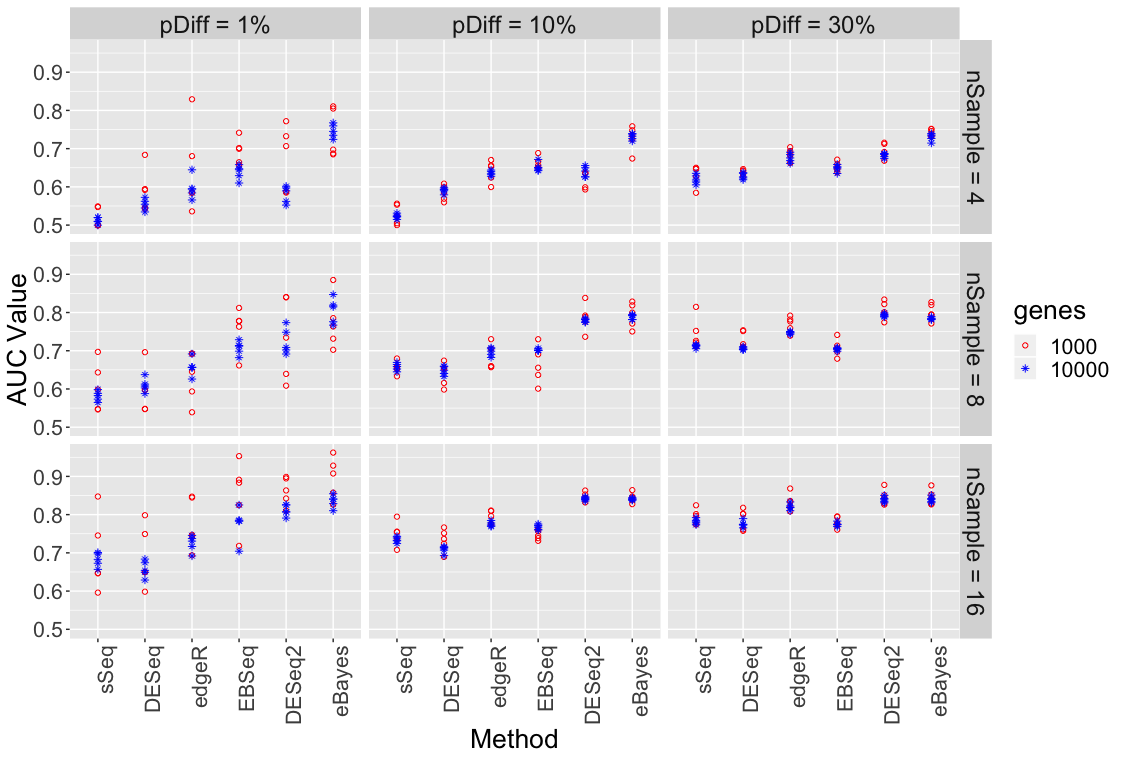
\includegraphics[height=10cm,width=18cm]{auc_plot}
\caption{AUC Plot of Simulated Datasets across Six Methods, Facetted by proportion of DE (pDiff) and number of samples (nSample), Colored by total number of Genes (nGenes)}
\label{auc}
\end{figure}

In terms of AUC values, ebayes method always have promising DE analysis performance.

When number of samples increases, AUC values of all methods increase. 

When DE proportion increases, the difference among the methods decreases. 

There is no obvious difference when number of genes differ.


\section{Discussion}










\renewcommand{\bibname}{\centerline{BIBLIOGRAPHY}}
\unappendixtitle
\newpage
\phantomsection
%\addcontentsline{toc}{chapter}{BIBLIOGRAPHY}
\bibliographystyle{plain}
\bibliography{mybib}

\appendixtitle 
\appendix
\section{Appendix}

\begin{figure}[h!tb] 
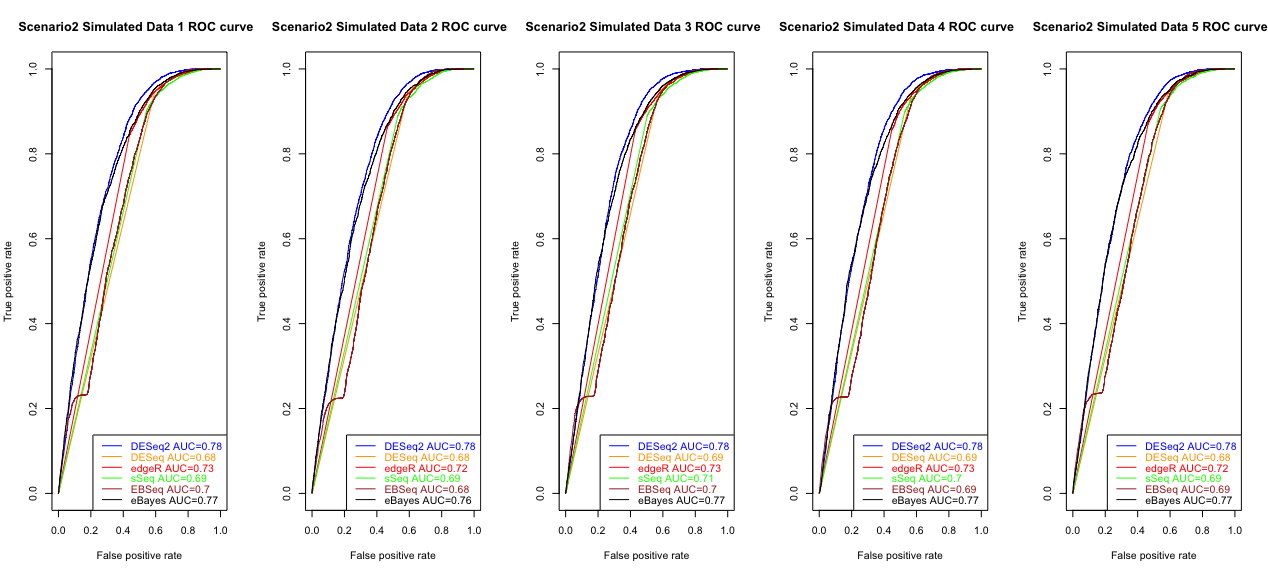
\includegraphics[height=6cm,width=15cm]{sc2_roc_curves}
\caption{ROC curves of Simulated Datasets with $nGenes=10000, nSamples=8, pDiff=30\%$}
\label{sc2_roc}
\end{figure}

\begin{figure}[h!tb] 
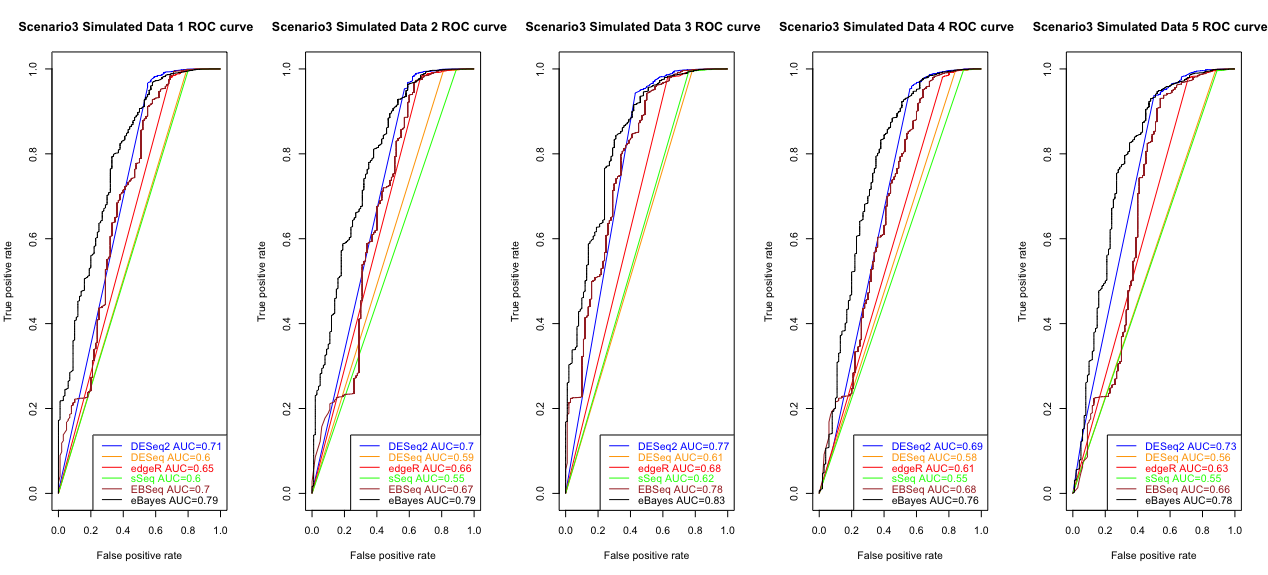
\includegraphics[height=6cm,width=15cm]{sc3_roc_curves}
\caption{ROC curves of Simulated Datasets with $nGenes=10000, nSamples=8, pDiff=1\%$}
\label{sc3_roc}
\end{figure}


\begin{figure}[h!tb] 
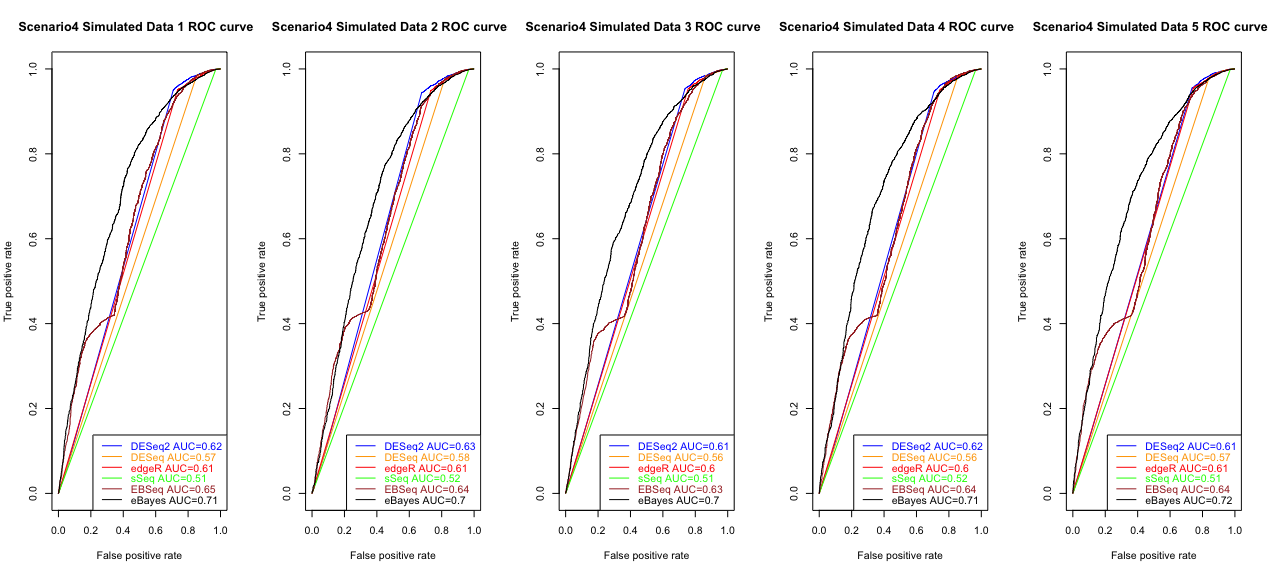
\includegraphics[height=6cm,width=15cm]{sc4_roc_curves}
\caption{ROC curves of Simulated Datasets with $nGenes=10000, nSamples=4, pDiff=10\%$}
\label{sc4_roc}
\end{figure}


\begin{figure}[h!tb] 
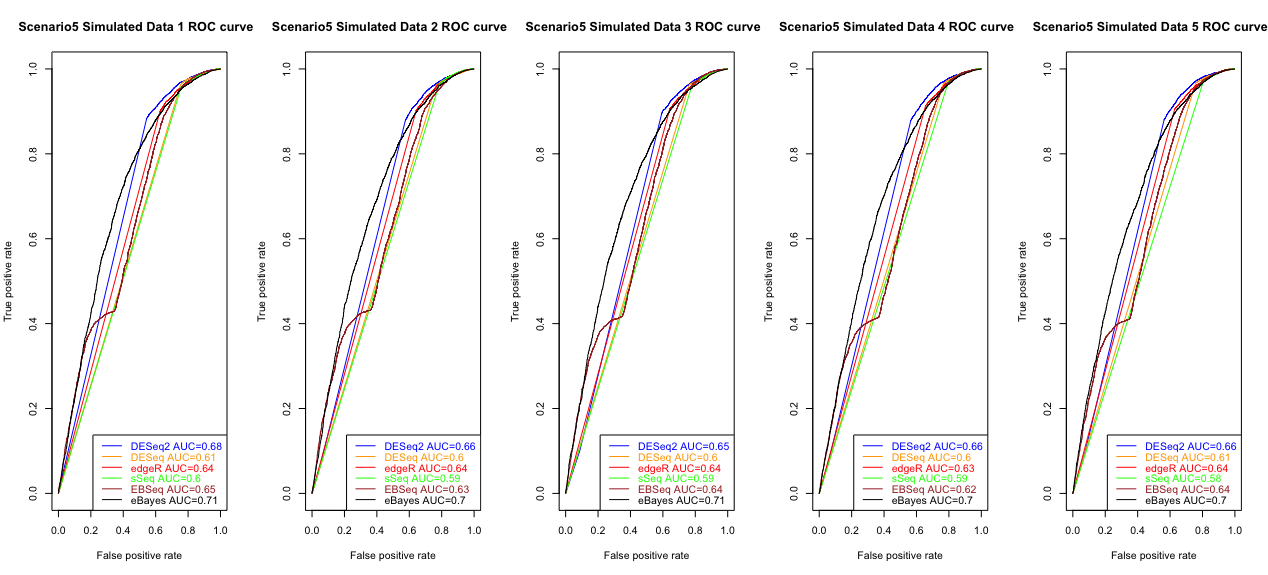
\includegraphics[height=6cm,width=15cm]{sc5_roc_curves}
\caption{ROC curves of Simulated Datasets with $nGenes=10000, nSamples=4, pDiff=30\%$}
\label{sc5_roc}
\end{figure}


\begin{figure}[h!tb] 
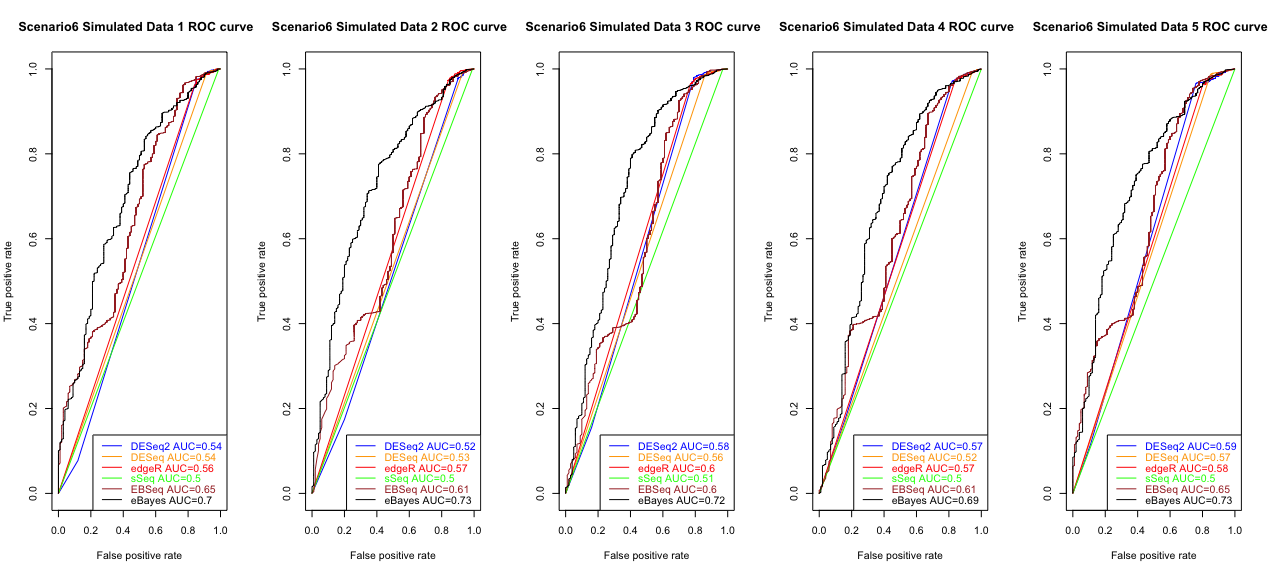
\includegraphics[height=6cm,width=15cm]{sc6_roc_curves}
\caption{ROC curves of Simulated Datasets with $nGenes=10000, nSamples=4, pDiff=1\%$}
\label{sc6_roc}
\end{figure}

\begin{figure}[h!tb] 
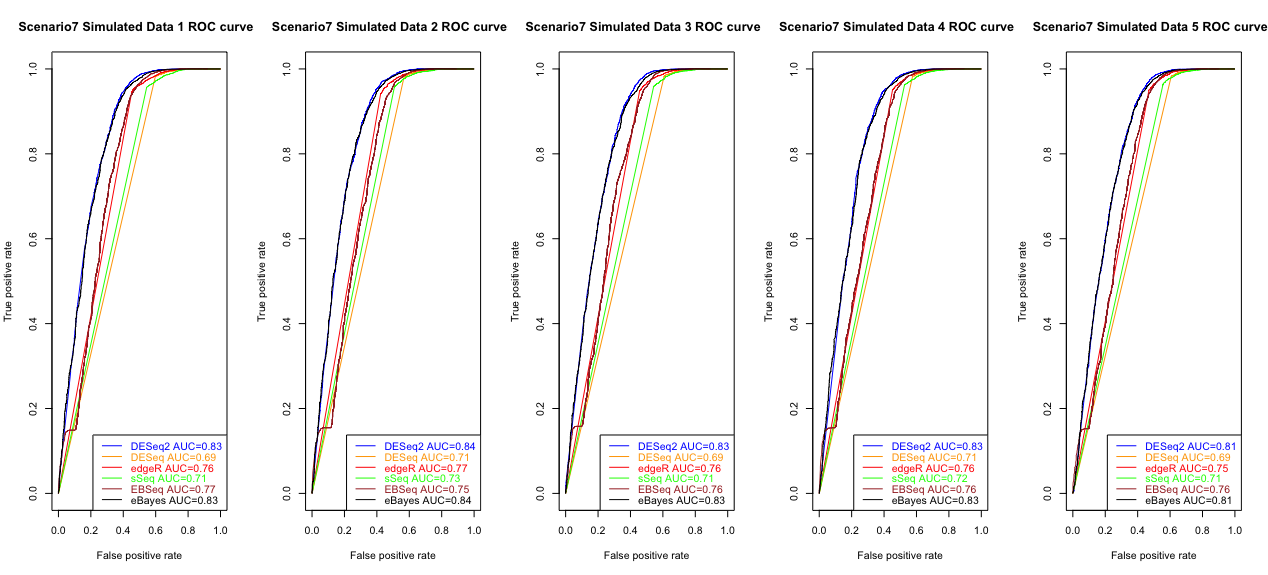
\includegraphics[height=6cm,width=15cm]{sc7_roc_curves}
\caption{ROC curves of Simulated Datasets with $nGenes=10000, nSamples=16, pDiff=10\%$}
\label{sc7_roc}
\end{figure}

\begin{figure}[h!tb] 
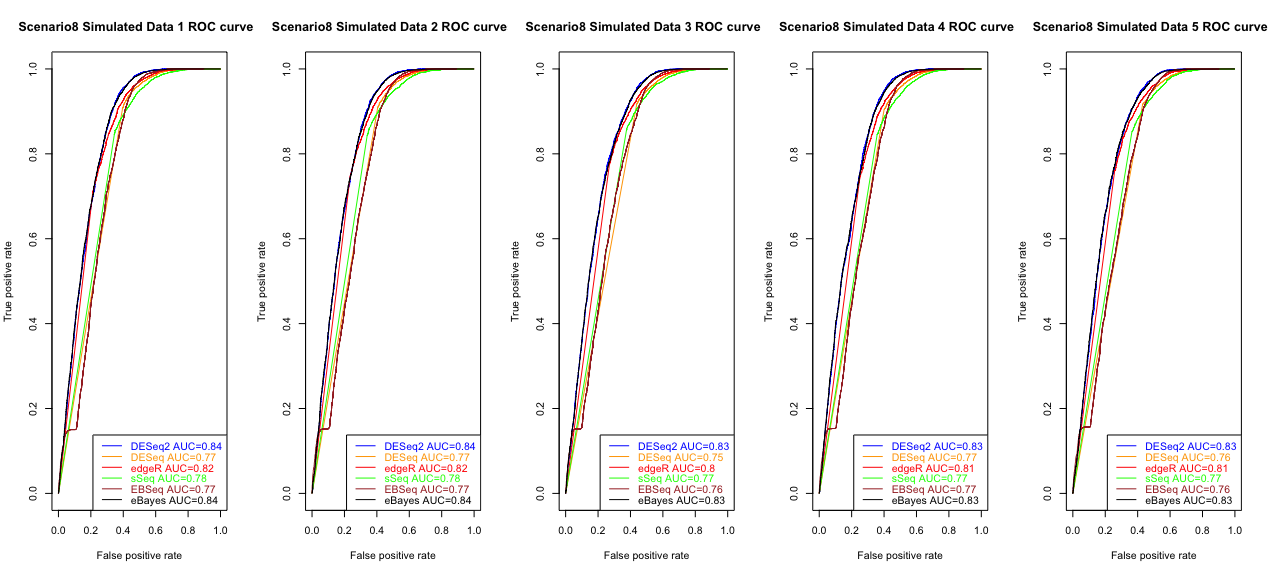
\includegraphics[height=6cm,width=15cm]{sc8_roc_curves}
\caption{ROC curves of Simulated Datasets with $nGenes=10000, nSamples=16, pDiff=30\%$}
\label{sc8_roc}
\end{figure}

\begin{figure}[h!tb] 
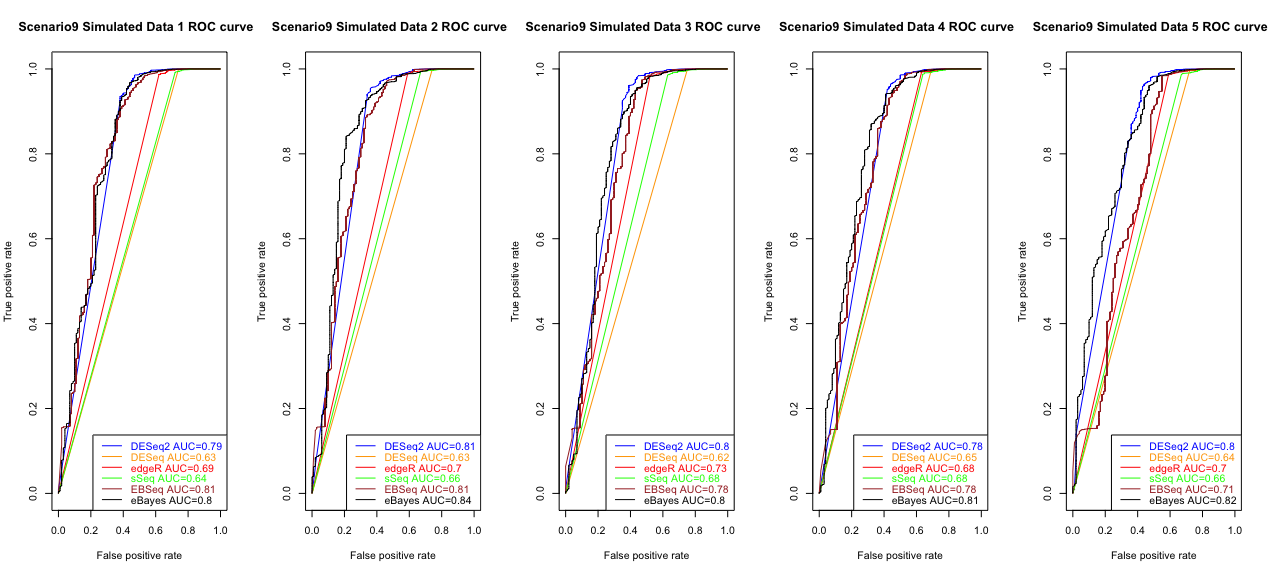
\includegraphics[height=6cm,width=15cm]{sc9_roc_curves}
\caption{ROC curves of Simulated Datasets with $nGenes=10000, nSamples=16, pDiff=1\%$}
\label{sc9_roc}
\end{figure}


\begin{figure}[h!tb] 
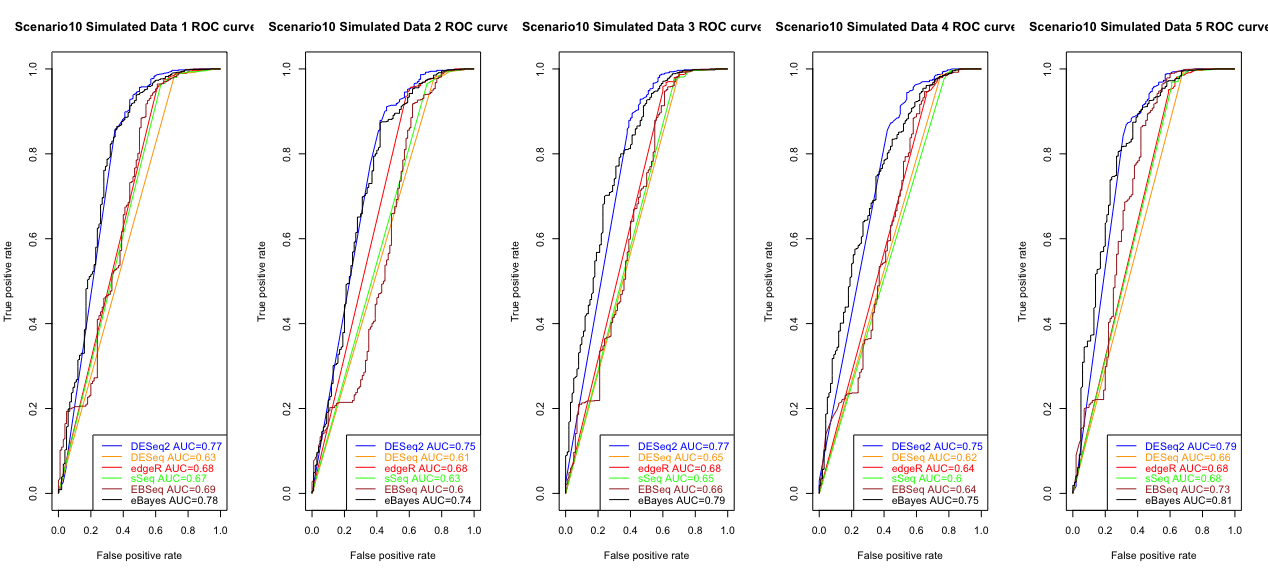
\includegraphics[height=6cm,width=15cm]{sc10_roc_curves}
\caption{ROC curves of Simulated Datasets with $nGenes=1000, nSamples=8, pDiff=10\%$}
\label{sc10_roc}
\end{figure}




\begin{figure}[h!tb] 
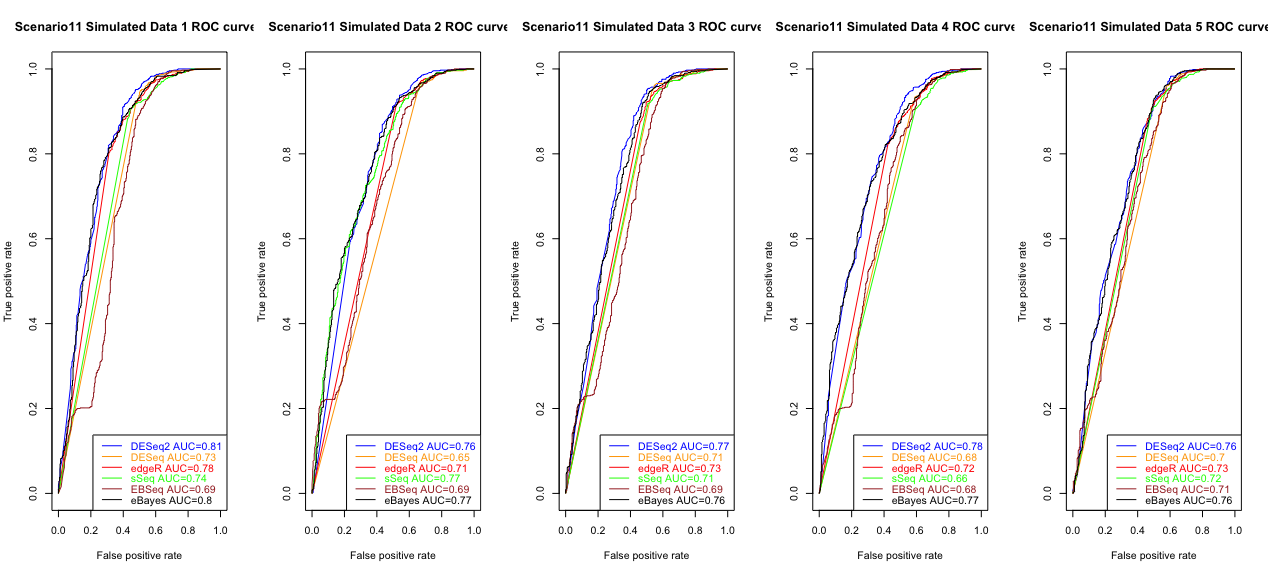
\includegraphics[height=6cm,width=15cm]{sc11_roc_curves}
\caption{ROC curves of Simulated Datasets with $nGenes=1000, nSamples=8, pDiff=30\%$}
\label{sc11_roc}
\end{figure}

\begin{figure}[h!tb] 
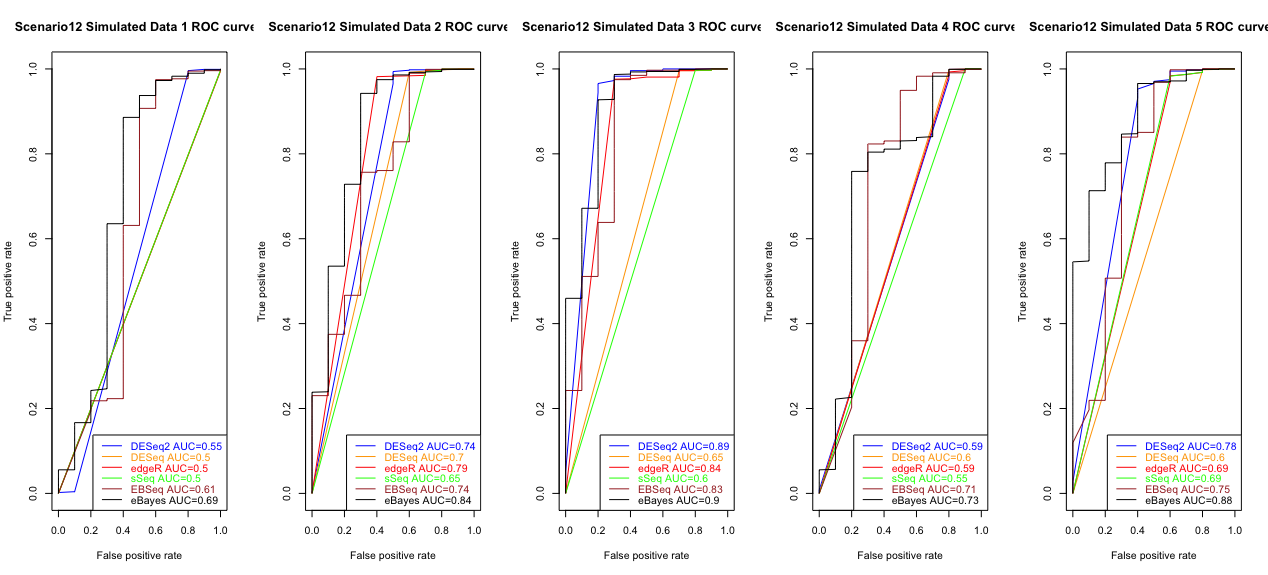
\includegraphics[height=6cm,width=15cm]{sc12_roc_curves}
\caption{ROC curves of Simulated Datasets with $nGenes=1000, nSamples=8, pDiff=1\%$}
\label{sc12_roc}
\end{figure}


\begin{figure}[h!tb] 
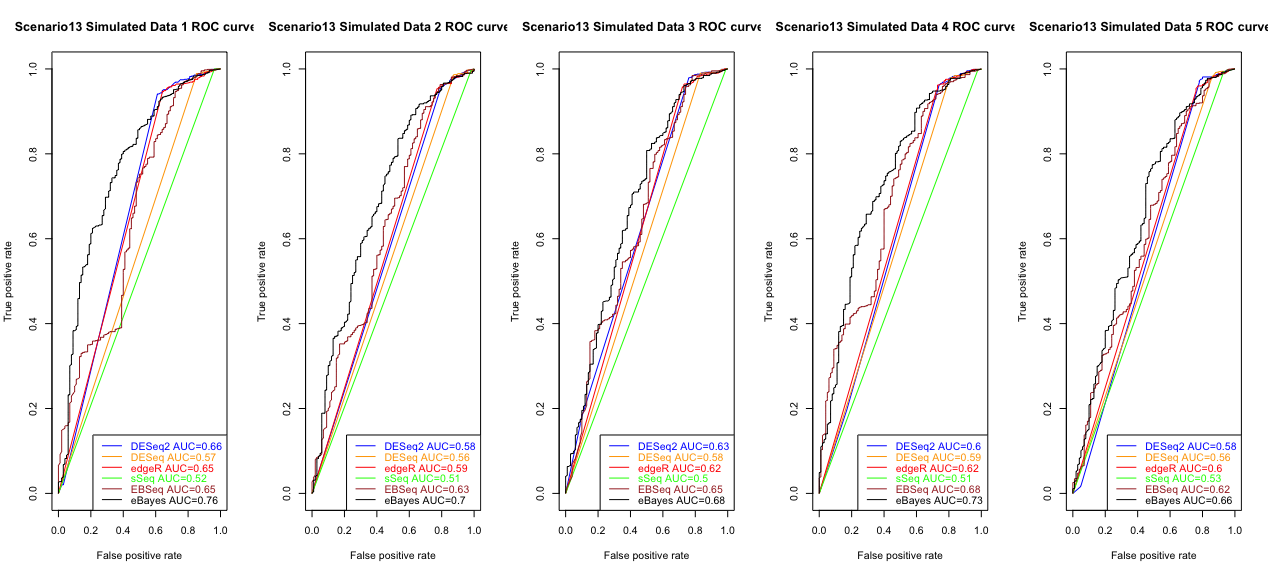
\includegraphics[height=6cm,width=15cm]{sc13_roc_curves}
\caption{ROC curves of Simulated Datasets with $nGenes=1000, nSamples=4, pDiff=10\%$}
\label{sc13_roc}
\end{figure}


\begin{figure}[h!tb] 
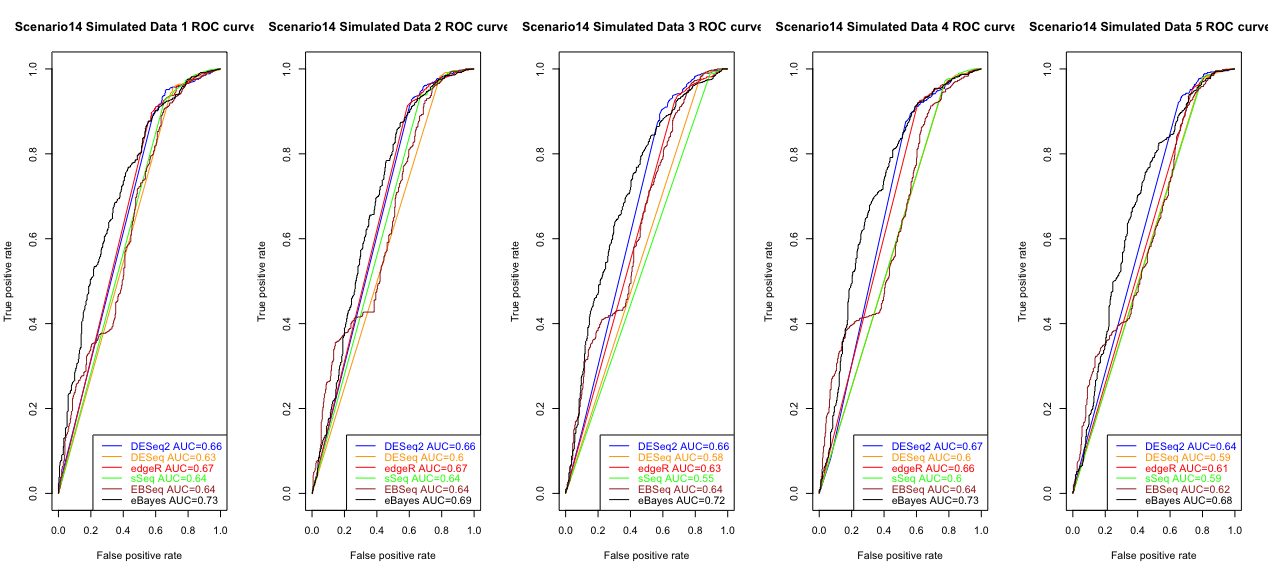
\includegraphics[height=6cm,width=15cm]{sc14_roc_curves}
\caption{ROC curves of Simulated Datasets with $nGenes=1000, nSamples=4, pDiff=30\%$}
\label{sc14_roc}
\end{figure}


\begin{figure}[h!tb] 
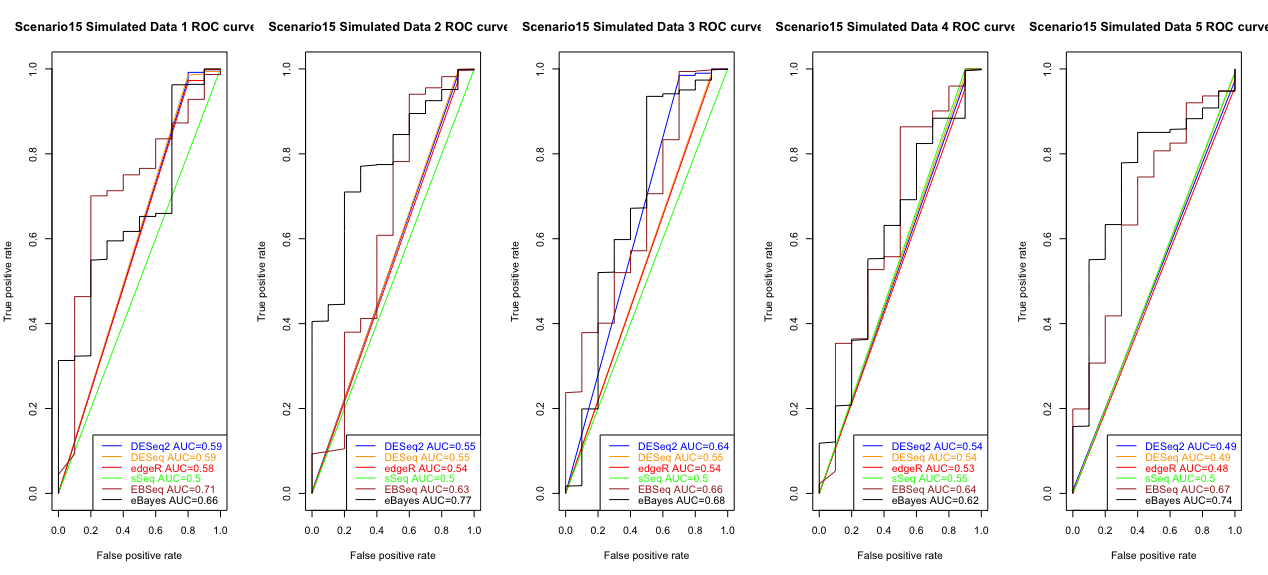
\includegraphics[height=6cm,width=15cm]{sc15_roc_curves}
\caption{ROC curves of Simulated Datasets with $nGenes=1000, nSamples=4, pDiff=1\%$}
\label{sc15_roc}
\end{figure}

\begin{figure}[h!tb] 
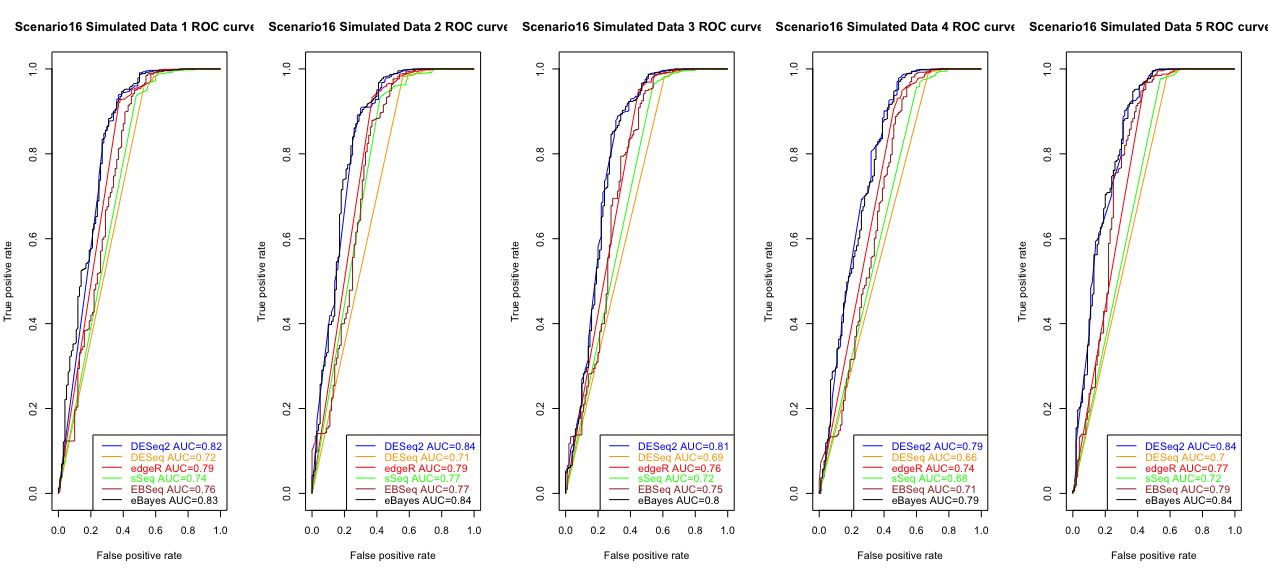
\includegraphics[height=6cm,width=15cm]{sc16_roc_curves}
\caption{ROC curves of Simulated Datasets with $nGenes=1000, nSamples=16, pDiff=10\%$}
\label{sc16_roc}
\end{figure}

\begin{figure}[h!tb] 
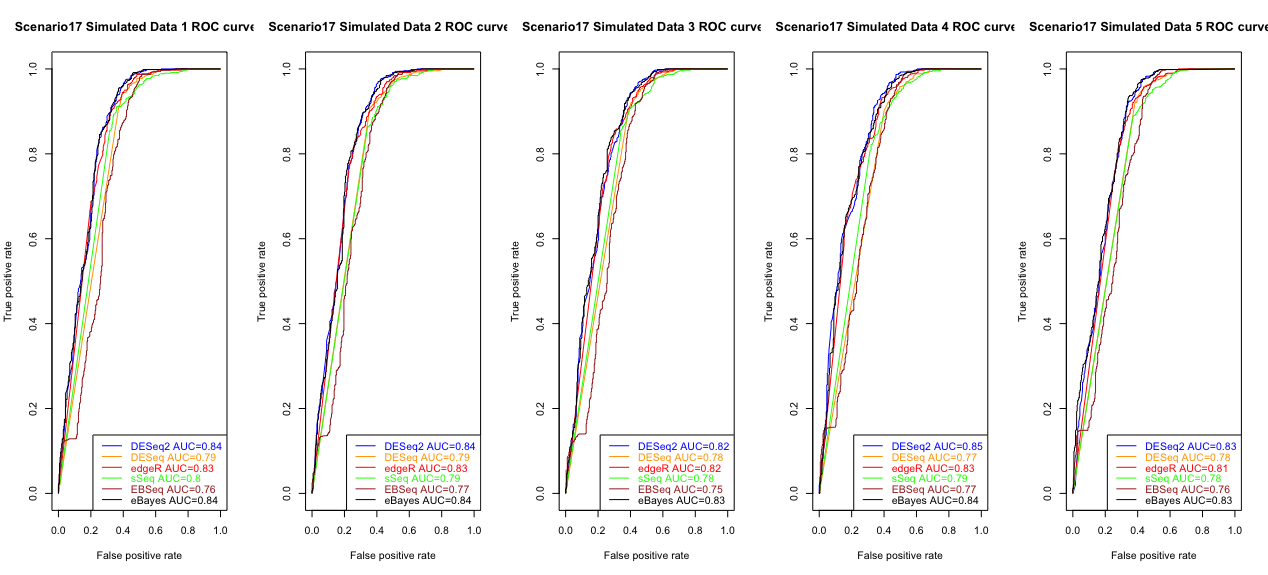
\includegraphics[height=6cm,width=15cm]{sc17_roc_curves}
\caption{ROC curves of Simulated Datasets with $nGenes=1000, nSamples=16, pDiff=30\%$}
\label{sc17_roc}
\end{figure}

\begin{figure}[h!tb] 
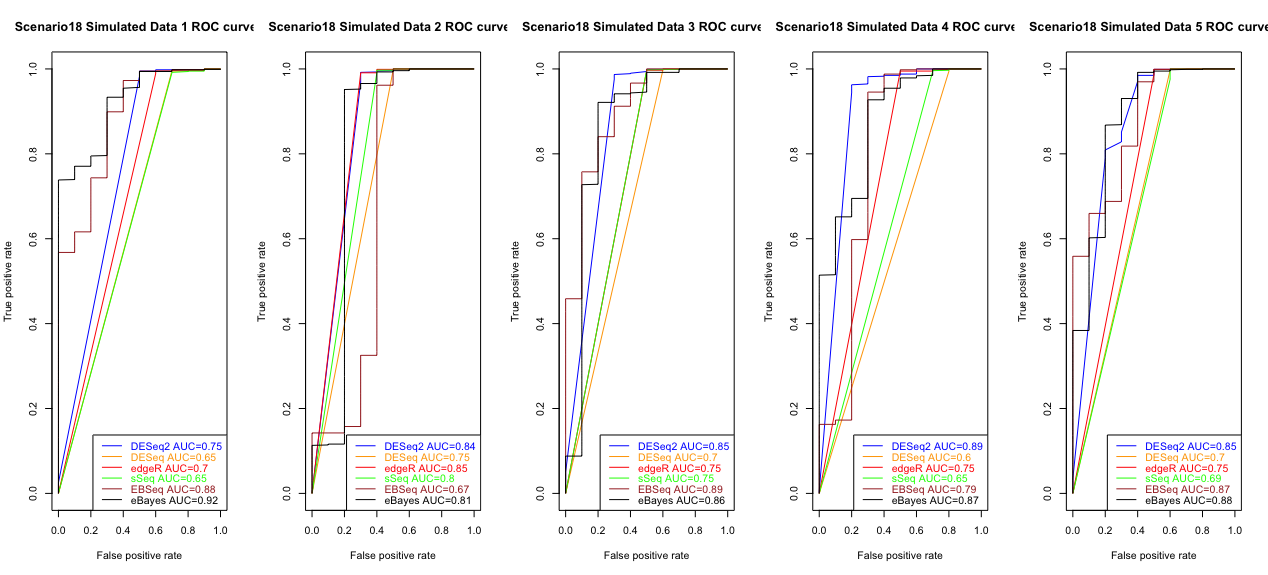
\includegraphics[height=6cm,width=15cm]{sc18_roc_curves}
\caption{ROC curves of Simulated Datasets with $nGenes=1000, nSamples=16, pDiff=1\%$}
\label{sc18_roc}
\end{figure}

\end{document}
